% !TEX root = main.tex
\chapter[head={The CKM angle $\gamma$},tocentry={The CKM angle $\symbfsf{\gamma}$}]{The CKM angle $\symbfsf{\gamma}$}
\label{ch:CKMAngleGamma}

As mentioned before overconstraining the triangle relations following from the unitarity of the matrix is a nice experimental self consistency check of the \ac{SM}.
The CKM angle $\gamma$ is one of five observables parametrising the CKM triangle described in \cref{eq:CKMtriangle}.
The current experimental constraints on this triangle are shown in \cref{fig:ckmtriangle}.
One can see that $\gamma$ is currently the least well known parameter.
Hence, a more accurate determination of $\gamma$ is one of the main tasks of current research in the field of flavour physics.
This chapter is organised as follows: Firstly it is described how $\gamma$ in general can be accessed in section \cref{sec:accessGamma}, especially the determination using tree-level decays (\cref{sec:gamamInTrees}) and loop-processes (\cref{sec:gamamInLoops}) is emphasized, followed by the explanation how the decay mode \BdToDpi can be used to derive constraints on $\gamma$ in \cref{sec:GammaInBd2Dpi}.

\begin{figure}[tbp]
	\centering
	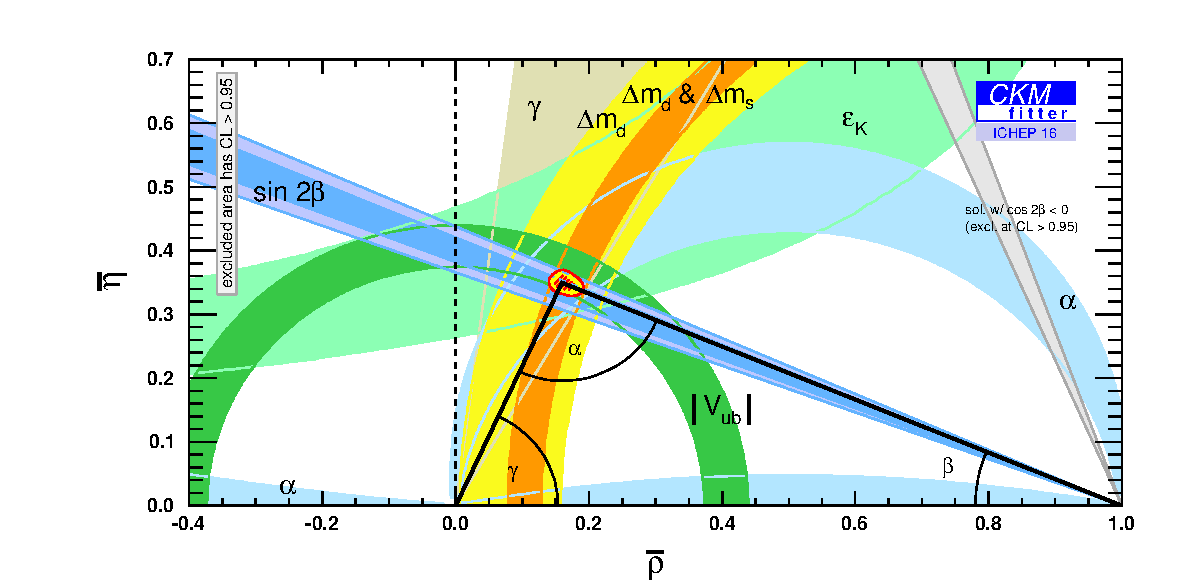
\includegraphics[width=0.8\textwidth]{04gamma/figs/CKMTriangle.pdf}
	\caption{CKM triangle in the complex plane.
	The coloured bands show the experimental constraints.
	The red hashed and the yellow area around the apex represent the currrent uncertainties at \SI{68}{\percent} and \SI{95}{\percent} confidence level, respectively~\cite{CKMfitter2015}.}
	\label{fig:ckmtriangle}
\end{figure}

\section[head={Accessing the angle $\gamma$},tocentry={Accessing the angle $\gamma$}]{Accessing the angle $\symbfsf{\gamma}$}
\label{sec:accessGamma}


As can be seen from the from in \cref{eq:CKMangles} the angle $\gamma$ is the only angle which is independent of CKM elements involving the top quark.
This makes it the only angle, which can be determined theoretically clean from tree-level decays.
On the other hand the experimental challenges are huge as transitions sensitive to $\gamma$ need to be proportional to \Vub, \ie such transitions are highly suppressed by order $\mathcal(O)\left(\lambda^3\right)$.
So either the precision of single measurements is limited due to small interference effects and branching fractions or in addition to the tree-level transition also penguin contributions of similar size contribute.
These gluonic penguins usually carry a weak phase different from the one in the tree-level diagram.

This latter possibility is briefly discussed using the example of the $\Bs\to\rho\KS$ decay.
Similar to the case of the golden mode \BdToJPsiKS, $\rho\KS$ is a \CP eigenstate and only the parameter \Lf needs to be calculated.
Using the amplitudes
\begin{equation}
\begin{aligned}
\Af&=\left<\rho\KS\left|T\right|\Bs\right>=-\frac{1}{2q_{\kaon}}\left<\rho\Kzb\left|T\right|\Bs\right>=-\frac{1}{2q_{\kaon}}\Vubst\Vud\\
\Abarf&=\left<\rho\KS\left|T\right|\Bsb\right>=\frac{1}{2p_{\kaon}}\left<\rho\Kz\left|T\right|\Bsb\right>=\frac{1}{2p_{\kaon}}\Vub\Vudst
\end{aligned}
\end{equation}
where $q_{\kaon}$ and $p_{\kaon}$ are the same mixing parameters for the neutral kaon system as shwon in \cref{eq:qoverp} for the \Bz-meson system.
With $\nicefrac{q_{\kaon}}{p_{\kaon}}=\nicefrac{\Vcsst\Vcd}{\Vcs\Vcdst}$ the parameter \Lf can be expressed in terms of the CKM matrix elements
\begin{equation}
\Lf=-\frac{q_{\kaon}}{p_{\kaon}}\frac{q}{p}\frac{\left<\rho\Kz\left|T\right|\Bsb\right>}{\left<\rho\Kzb\left|T\right|\Bs\right>}
=-\frac{\Vcsst\Vcd}{\Vcs\Vcdst}\frac{\Vtbst\Vts}{\Vtb\Vtsst}\frac{\Vub\Vudst}{\Vubst\Vud}.
\end{equation}
Using the Wolfenstein paramtrisation as shown in \cref{eq:CKMmatrix} this simplifies \Lf being a pure phase
\begin{equation}
\Lf=e^{-2i\gamma}.
\end{equation}
For $\Bs\to\rho\KS$ the finalstate $\rho$ has a \uquark\uquarkbar and a \dquark\dquarkbar component.
This means that alongside the spectator \squark-quark not only the tree-level transition $\bquark\to\uquark\uquarkbar\dquarkbar$ but also the gluonic-penguin transition $\bquark\to\dquark\dquarkbar\dquarkbar$ is possible (see \cref{fig:Bs2RhoKS}).
\begin{figure}[tbp]
	\centering
	\includestandalone{04gamma/figs/BsToRhoKS_Tree}
	\includestandalone{04gamma/figs/BsToRhoKS_Penguin}
	\caption{Tree-level diagram of $\Bs\!\to\rho\KS$ (left) and the dominantly contributing gluonic penguin (right). \cite{Ellis:2016jkw}.}
	\label{fig:Bs2RhoKS}
\end{figure}
For both diagrams the CKM-factor is $\propto A\lambda^3$, but the weak phases are $\gamma$ and $\beta$ for the tree-level diagram and the penguin, respectively.
The effect of an additional contributing amplitude with a weak phase differing from the one of the tree-level process can be quantified.
Considering two weak phases contributing to the transitions \Af ($\Bs\to\rho\KS$) and \Abarf ($\Bsb\to\rho\KS$):
\begin{equation}
\begin{aligned}
\Af&=A_1e^{i\left(\Phi_{A_1}+\delta_1\right)}+A_2e^{i\left(\Phi_{A_2}+\delta_2\right)}\\
\Abarf&=\eta_f\left[A_1e^{i\left(-\Phi_{A_1}+\delta_1\right)}+A_2e^{i\left(-\Phi_{A_2}+\delta_2\right)}\right]
\end{aligned}
\end{equation}
As shown in \cref{eq:qoverPPurePhase} the quantity $\nicefrac{q}{p}$ is a pure phase and hence one can write $\nicefrac{q}{p}=-e^{2i\Phi_\text{M}}$, what leads to
\begin{equation}
\Lf=-\eta_f\,e^{2i\Phi_\text{M}}\frac{ A_1 e^{i\left(-\Phi_{A_1}+\delta_1\right)} + A_2 e^{i\left(-\Phi_{A_2}+\delta_2\right)}}{A_1e^{i\left(\Phi_{A_1}+\delta_1\right)}+A_2e^{i\left(\Phi_{A_2}+\delta_2\right)}} \label{eq:LfWithPenguin}
\end{equation}
with the \emph{weak} and \emph{strong} phases $\Phi_{A_i}$ and $\delta_i$, respectively.
The phases $\Phi_{A_1}$, $\Phi_{A_2}$ and $\Phi_\text{M}$ are not rephasing-invariant, but the relative phases $\Phi_1\equiv\Phi_{A_1}-\Phi_\text{M}$, $\Phi_2\equiv\Phi_{A_2}-\Phi_\text{M}$ and $\Delta=\delta_2-\delta_1$ can be measured.
For $\Bs\to\rho\KS$ one can \eg identify $A_1$ and $A_2$ with amplitude corresponding to the tree-level and gluonic-penguin diagram, respectively.
Accordingly the phase $\Phi_1$ and $\Phi_2$ would represent the CKM angles $\gamma$ and $\beta$.
Already the form of $\Lf$ in \cref{eq:LfWithPenguin} shows that the penguin contribution in $\Bs\to\rho\KS$ makes it impossible to measure $\gamma$
However this case might be extrem in the sense that both amplitudes are of the same magnitude.
But even with the approximation that $r=\nicefrac{A_2}{A_1}$ is small one finds
\begin{align}
\Lf&=-\eta_fe^{-2i\Phi_1}\frac{1+re^{i\left(\Delta-\Phi_2+\Phi_1\right)}}{1+re^{i\left(\Delta+\Phi_2-\Phi_1\right)}}\nonumber\\
&\approx-\eta_fe^{-2i\Phi_1}\left[1+2r\sin\Delta\sin\left(\Phi_2-\Phi_1\right)-2ir\cos\Delta\sin\left(\Phi_2-\Phi_1\right)\right].
\end{align}
Obviously in case a guonic-penguin contributes with a different weak phase from that of the tree-level diagram - \ie $r\neq0$ and $\Phi_1\neq\Phi_2$ - it is not possible to measure a single weak phase.
Now one finds, that in case a second penguin with a different weak phase from that of the tree-level diagram contributes the parameter and $r\neq0$, \Lf does not allow to measure a single weak phase.
Even in the case of vanishing final state interactions, \ie $\Delta=0$, \Lf can just be written as
\begin{equation}
\Lf=-\eta_fe^{-2i\left(\Phi_1-\delta_{\Phi_1}\right)}
\end{equation}
where $\delta_{\Phi_1}$ is defined by
\begin{equation}
\tan\left(\delta_{\Phi_1}\right)=\frac{r\sin\left(\Phi_1-\Phi_2\right)}{1+r\cos\left(\Phi_1-\Phi_2\right)}.
\end{equation}
Additionally it is important to note that hadronic matrix elements cannot be calculated reliably.
This means that in case they do not cancel out as they do if only one amplitude contributes to a specific decay, the resulting \CP asymmetries cannot be interpreted without large uncertainties which need to be propagated into the determination of the sides and angles of the unitarity triangle.

Therefore the current strategy to decrease the uncertainty on $\gamma$ is to measure it in many different decay modes and combine the results afterwards.
These decay modes can be divided into the two mentioned classes: The first class are tree-level processes where either decays of charged \B mesons or neutral \B mesons are exploited.
The second class are processes involving penguin contributions, \eg similar to the contribution to $\Bs\to\rho\KS$ described above.

\subsection[head={Determination of $\gamma$ in tree-level decays},tocentry={Determination of $\gamma$ in tree-level decays}]{Determination of $\symbfsf{\gamma}$ in tree-level decays}
\label{sec:gamamInTrees}

% In the \ac{SM} two types of \CP violation, namely direct and interference \CP violation, are expected to a non-negligible amount.
As $\gamma$ is propotional to the phase of the matrix element \Vub a natural way to measure it is to exploit interference effects between the Cabibbo-favoured $\bquark\to\cquark$ transitions and the Cabibbo-suppressed $\bquark\to\uquark$ transitions in decay channels such as $\Bu\to\D\Kp$ and \BsToDsK.
In the first case exploring different \D decay chaines requires slightly different experimental methods, whereas in the latter case a time-dependent analysis is needed.

The basic principle when exploiting decays of charged \B mesons is always the same.
The initial \Bpm meson decays into \Dz\Kpm or \Dzb\Kpm and subsequently the \D meson is reconstructed in a final state common to both \Dz and \Dzb.
Therefore the amplitudes for the decay of the \B meson can be defined as
\begin{equation}
\begin{aligned}
A\!\left(\Bp\!\to\Dz\Kp\right)&=\Vubst\Vcs=Ae^{i\left(\delta+\gamma\right)}\\
A\!\left(\Bp\!\to\Dzb\Kp\right)&=\Vcbst\Vus=\overline{\kern -1.0pt A\kern -1.0pt}\,e^{i\left(\overline{\delta}\right)}
\end{aligned}
\end{equation}
where the \emph{weak} phase was directly idenitified as $\gamma$, $\delta$ and $\overline{\delta}$ are the \emph{strong} phases and $A$ and $\overline{\kern -1.0pt A\kern -1.0pt}$ are the moduli of the amplitudes.
For the \D-meson decay the ampltiudes can be defined accordingly as
\begin{equation}
\begin{aligned}
A\!\left(\Dz\!\to\f\right)&=A_De^{i\left(\delta_D\right)}\\
A\!\left(\Dzb\!\to\f\right)&=\overline{\kern -1.0pt A\kern -1.0pt}_D\,e^{i\left(\overline{\delta}_D\right)}.
\end{aligned}
\end{equation}
Hence, the transition of $\Bp\to\f$ has two contributing amplitudes, which produce an interference term containing $\gamma$ in the total decay rate
\begin{equation}
\left|A\!\left(\Bp\!\to\f\,\Kp\right)\right|^2=A^2\overline{\kern -1.0pt A\kern -1.0pt}{}_D^2\left(1+r_\B^2r_\D^2+2\,r_\B r_\D\cos\left(\Delta+\Delta_\D+\gamma\right)\right)\label{eq:totDecRateChargedB}
\end{equation}
where the short notations $r_\B=\nicefrac{\overline{\kern -1.0pt A\kern -1.0pt}}{A}$, $r_\D=\nicefrac{A_\D}{\overline{\kern -1.0pt A\kern -1.0pt}_\D}$, $\Delta=\overline{\delta}-\delta$ and $\Delta_\D=\delta_\D-\overline{\delta}_\D$ were used.
To obtain the total decay rate for the \Bm decay just the sign of $\gamma$ must be reversed.

The first method exploiting this interference is the so-called GLW method \cite{GLW_1, GLW_2}.
The ideas is simply to reconstruct the intermediate \D meson in \CP eigenstates such as \Kp\Km (\CP-even) or \KS\piz (\CP-odd).
The consequences of such choice are that the unknowns from the \D decay can be reduced because $r_\D=1$ and $\Delta_\D=0$, so the total decay rates for \eg a \CP-even \D decay can be written as
\begin{equation}
\left|A\!\left(\Bpm\!\to f_{\CP}\Kpm\right)\right|^2=A^2A_\D^2\left(1+r_\B^2+2r_\B\cos\left(\Delta\pm\gamma\right)\right).\label{eq:totDecRateGLW}
\end{equation}
Experimentally for the \CP-even final state a \CP asymmetry
\begin{equation}
A_{\CP}^{\text{GLW}}=\frac{\left|A\!\left(\Bm\!\to f_{\CP}\Km\right)\right|^2-\left|A\!\left(\Bp\!\to f_{\CP}\Kp\right)\right|^2}{\left|A\!\left(\Bm\!\to f_{\CP}\Km\right)\right|^2+\left|A\!\left(\Bp\!\to f_{\CP}\Kp\right)\right|^2}=\frac{2r_\B\sin\left(\Delta\right)\sin\left(\gamma\right)}{1+r_\B^2+2r_\B\cos\left(\Delta\pm\gamma\right)}\label{eq:ACP_GLW}
\end{equation}
and a \CP ratio
\begin{equation}
R_{\CP}^{\text{GLW}}=\frac{\left|A\!\left(\Bm\!\to f_{\CP}\Km\right)\right|^2+\left|A\!\left(\Bp\!\to f_{\CP}\Kp\right)\right|^2}{2\left|A\!\left(\Bm\!\to\Dz\Km\right)\right|^2}=1+r_\B^2+2r_\B\cos\left(\Delta\right)\cos\left(\gamma\right)\label{eq:RCP_GLW}
\end{equation}
can be measured. If the \D meson in the denominator of $R_{\CP}^{\text{GLW}}$ is reconstructed in a hadronic final state as \kaon\pion decays proceeding via a \Dz or a \Dzb cannot distinguished as both decay into \Kp\pim and \Km\pip. However, this can be avoided by measuring instead the double ratio
\begin{equation}
R_{+}^{\text{GLW}}=\frac{\left|A\!\left(\Bm\!\to f_{\CP}\Km\right)\right|^2+\left|A\!\left(\Bp\!\to f_{\CP}\Kp\right)\right|^2}{\left|A\!\left(\Bm\!\to f_{\CP}\pim\right)\right|^2+\left|A\!\left(\Bp\!\to f_{\CP}\pip\right)\right|^2}\times\frac{1}{R_{\kaon/\pion}}
\end{equation}
with
\begin{equation}
R_{\kaon/\pion}=\frac{\left|A\!\left(\Bm\!\to \D\left(\to\Km\pip\right)\Km\right)\right|^2+\left|A\!\left(\Bp\!\to \D\left(\to\Kp\pim\right)\Kp\right)\right|^2}{\left|A\!\left(\Bm\!\to \D\left(\to\Km\pip\right)\pim\right)\right|^2+\left|A\!\left(\Bp\!\to \D\left(\to\Kp\pim\right)\pip\right)\right|^2}.
\end{equation}
This double ratio $R_{+}^{\text{GLW}}$ is identical to $R_{\CP}^{\text{GLW}}$ when neglecting all terms proportional to $r_\D$ or $r_{\B_\pion}=\nicefrac{A\!\left(\Bp\!\to\Dz\pip\right)}{A\!\left(\Bm\!\to\Dz\pim\right)}$.
However the GLW method has two disadvantages: Firstly, the interference term is proportional to $r_\B$ which is of order \SI{10}{\percent} and therefore decreases the sensitivity on $\gamma$.
Second, there is not only one solution for $\gamma$, but there is a eight-fold discrete ambiguity due to the fact that $\gamma$ and $\Delta$ always appear together in the product of two sine or cosine functions as in \cref{eq:ACP_GLW} and \cref{eq:RCP_GLW}.

The second method directly counteracts to the first disadvantage of the GLW method.
Instead of using decays into \CP-eigenstates of the \D meson, the \D is reconstructed in a final state for which $\Dz\!\to\f$ is suppressed relative to $\Dzb\!\to\f$ (\eg \f could be \Km\pip) \cite{ADS}.
This enhances the interference term to be of the same order as the other ones, but on the other hand the $r_\D$ and $\Delta_\D$ do not cancel as before.
Hence, to determine $\gamma$ from similar asymmetries and ratios as for the GLW method external input for both quantities is needed.

The last method described in this section using charged \B decays is probably the most sophisticated one.
The GGSZ method makes use of multibody \D decays.
This requires an analysis of the Dalitz plane, but on the other hand $\gamma$ can be extracted without the disadvantages of the GLW or the ADS method.
The basic idea however is the same as before, just that the strong phase originating from the \D decay varies over the Dalitz plane.
Furthermore, the interference term can be expressed in the form $\cos\!\left(\phi\right)c_i\pm\sin\!\left(\phi\right)s_i$, where $\phi$ is the difference (sum) of the \emph{strong} phase $\delta_\B$ originating from the \Bm (\Bp) decay and $\gamma$.
The coefficients $c_i$ and $s_i$ contain the \emph{strong} phases from the \D decay.
Using $k$ pairs of bins which are symmetrically around the $m_{\KS\pim}\leftrightarrow m_{\KS\pip}$ line in the Dalitz plot, and exploiting the symmetry of the $c_i$ and $s_i$ around this line leads to $4k$ equations.
This equations are related to the $2k+3$ unknowns $c_i$, $s_i$, $r_\B$, $\delta_\B$ and $\gamma$, so that a partition of the \D meson Dalitz plot into four or more bins allows to determine all unknowns.

Finally it is important to note, that the described techniques can be applied as well to any decays of type $\Bpm\!\to\D X^{\pm}$ where X is any state with the flavour of a \Kpm.

When exploiting decays of uncharged \B mesons such as \BsToDsK or \BdToDpi to determine the angle $\gamma$ the procedure is different.
This type of decays is only affected by interference \CP violation and therefore a time-dependent analysis is needed to achieve sensitivity at $\gamma$.
The basic formalism is already described in \cref{sec:formulaeCPV}.
Due to the \CP conservation in the decay, $\Cfbar=-\Cf$ and the number of independent coefficients as given in \cref{eq:cpcoeff} and \cref{eq:cpcoeffbar} is reduced to five.
Furthermore the \CP coefficient \Cf contains the ratio $r_\B$, while via the coefficients \Sf, \Sfbar, $A_f^{\DG}$, $A_{\kern 1.5pt\overline{\kern -1.5pt f\kern 1.5pt}}^{\DG}$ the phase information are measurable.
This experimental technique to measure \CP violation can be also applied to \BdToDpi and therefore it will be described more thouroughly in \cref{sec:GammaInBd2Dpi}.

\subsection[head={Determination of $\gamma$ in loop processes},tocentry={Determination of $\gamma$ in loop processes}]{Determination of $\symbfsf{\gamma}$ in loop processes}
\label{sec:gamamInLoops}
Instead of exploiting decays where $\gamma$ can be accessed via the interference in tree-level diagrams between the transitions $\bquark\to\uquark$ and $\bquark\to\cquark$ also processes containing loop transitions can be used to infer information about $\gamma$.
The first and probably most obvious possibility is to derive a result for $\gamma$ from experimental mesaurements of other CKM triangle quantities as the remaining two angles of the CKM triangle, $\alpha$ and $\beta$.
As an example the angle $\beta$ can be measured quite precisely in the decay \BdToJPsiKS while the angle $\alpha$ is accessible via Isospin analyses of the decays $\Bd\!\to\pip\pim$, $\Bd\!\to\piz\piz$ and $\Bu\!\to\pip\piz$ \cite{IsospinAlpha} or measurements of longitudinally polarized $\Bz\!\to\rho\rho$ decays \cite{alpha_BaBar, alpha_Belle}. Though, the best precision is achieved performing a \emph{full} fit using all available inputs as performed by the CKMfitter and UTfit collaborations \cite{CKMfitter2015, UTfit-UT}.

However such tests of a closing CKM triangle do not directly indicate certain processes that are affected effects of \ac{NP}.
Therefore, a more direct determination of $\gamma$ is also important.
A possibility for such determination is to extract $\gamma$ from \CP violation measurements in $B\!\to\pion\pion$ and $\Bs\!\to\Kp\Km$ \cite{GammaInLoops_Fleischer, GammaInLoops_Ciuchini}.
To do this, the U-spin flavour symmetry of strong interactions between the two decay channels - \ie the decays are related by interchanging all \dquark-quarks with \squark-quarks - must be used.
\begin{figure}[tbp]
	\centering
	\includestandalone{04gamma/figs/GammaLoopsTree}
	\hfill
	\includestandalone{04gamma/figs/GammaLoopsPenguin}
	\caption{Feynman diagrams contributing to $\Bd\!\to\pip\pim$ ($\quark=\dquark$) and $\Bs\!\to\Kp\Km$($\quark=\squark$) \cite{Ellis:2016jkw}.}
	\label{fig:feynmanGammaLoops}
\end{figure}

To briefly outline the strategy first the transition amplitudes and \CP observables for the decay modes $\Bz\!\to\pip\pim$ and $\Bs\!\to\Kp\Km$ will be introduced in the following:
In \cref{fig:feynmanGammaLoops} the dominant $\bquark\!\to\uquarkbar\uquark\dquarkbar$ processes are shown, which leads to the transition amplitude
\begin{equation}
A\!\left(\Bd\!\to\pip\pim\right)=\lambda_\uquark\left(A_{\text{cc}}^\uquark+A_{\text{pen}}^\uquark\right)+\lambda_\cquark A_{\text{pen}}^\cquark+\lambda_\tquark A_{\text{pen}}^\tquark
\end{equation}
where the amplitudes $A_{\text{pen}}^\quark$ and $A_{\text{c}}^\quark$ describe the penguin and charged-current contributions respectively.
Furthermore the short notation $\lambda_\quark=V_{{\kern -0.1em}\quark\dquark}V^{*}_{{\kern -0.1em}\quark\bquark}$ was used.
Making use of the unitarity of the CKM matrix and applying the Wolfenstein parametrisation \cite{Wolfenstein:1983yz} allows to determine the parameter \Lf and the corresponding \CP coefficients
\begin{equation}
\begin{aligned}
C_{f}^{\Bd\!\to\pip\pim}&=-\left[\frac{2d\sin\!\left(\theta\right)\sin\!\left(\gamma\right)}{1-2d\cos\!\left(\theta\right)\cos\!\left(\gamma\right)+d^2}\right]\\
S_{f}^{\Bd\!\to\pip\pim}&=\left[\frac{\sin\!\left(2\beta+2\gamma\right)-2d\cos\!\left(\theta\right)\sin\!\left(2\beta+\gamma\right)+d^2\sin\!\left(2\beta\right)}{1-2d\cos\!\left(\theta\right)\cos\!\left(\gamma\right)+d^2}\right].
\end{aligned}
\end{equation}
The quantities $d$ and $\theta$ are defined as
\begin{equation}
de^{i\theta}=\frac{1}{\left(1-\nicefrac{\lambda^2}{2}\right)R_b}\left(\frac{A_{\text{pen}}^{\cquark\tquark}}{A_{\text{cc}}^{\uquark}+A_{\text{pen}}^{\uquark\tquark}}\right)
\end{equation}
with $A_{\text{pen}}^{\quark\tquark}=A_{\text{pen}}^{\quark}-A_{\text{pen}}^{\tquark}$ and the CKM factor $R_b=\nicefrac{1}{\lambda}\left|\nicefrac{\Vub}{\Vcb}\right|$.
The \CP coefficient $A_f^{\DG}$ is neglected as the decay width difference for \Bd mesons is expected to be negligibly small.

Equivalent to this, the \CP coefficients for $\Bs\!\to\Kp\Km$ can be calculated as
\begin{equation}
\begin{aligned}
C_{f}^{\Bs\!\to\Kp\Km}&=\left[\frac{2\tilde{d'}\!\sin\!\left(\theta'\right)\sin\!\left(\gamma\right)}{1-2\tilde{d'}\!\cos\!\left(\theta'\right)\cos\!\left(\gamma\right)+\tilde{d'}^2}\right]\\
S_{f}^{\Bs\!\to\Kp\Km}&=\left[\frac{\sin\!\left(\phi_\squark+2\gamma\right)-2\tilde{d'}\!\cos\!\left(\theta\right)\sin\!\left(\phi_\squark+\gamma\right)+\tilde{d'}{}^2\!\sin\!\left(\phi_\squark\right)}{1-2\tilde{d'}\!\cos\!\left(\theta'\right)\cos\!\left(\gamma\right)+\tilde{d'}{}^2}\right]\\
A_f^{\DG, \Bs\!\to\Kp\Km}&=-\left[\frac{\cos\!\left(\phi_\squark+2\gamma\right)+2\tilde{d'}\!\cos\!\left(\theta'\right)\cos\!\left(\phi_\squark+\gamma\right)+\tilde{d'}{}^2\cos\!\left(\phi_\squark\right)}{1-2\tilde{d'}\!\cos\!\left(\theta'\right)\cos\!\left(\gamma\right)+\tilde{d'}{}^2}\right]
\end{aligned}
\end{equation}
where the short notation $\tilde{d'}=\left(\nicefrac{1-\lambda^2}{\lambda^2}\right)d'$ was used.
Assuming the U-spin flavour symmetry to be exact even implies that $d'=d$ and $\theta'=\theta$.

This theoretical setup can now be used in several strategies to determine $\gamma$ among other observables as $\beta$, $d$ and $\theta$.
In the following the basic idea of most strategies will be outlined briefly.
In the first approach the phase $\phi_s$ is taken as an external input, thus the four unknows $d$, $\theta$, $\beta$ and $\gamma$ can be determined using only the four observables $C_{f}^{B\!\to hh}$, and $S_{f}^{B\!\to hh}$.
As shown in \cite{GammaInLoops_Fleischer}, the coefficient the parameters $d$ and $\theta$ can be expressed as functions of $\gamma$, $C_{f}^{\Bs\!\to\Kp\Km}$ and $S_{f}^{\Bs\!\to\Kp\Km}$.
Inserting this into $C_{f}^{\Bd\!\to\pip\pim}$ allows then to determine $\gamma$ up to a two-fold ambiguity as shown in \cref{fig:gamma_beta_fleischer}.
\begin{figure}[tbp]
	\centering
	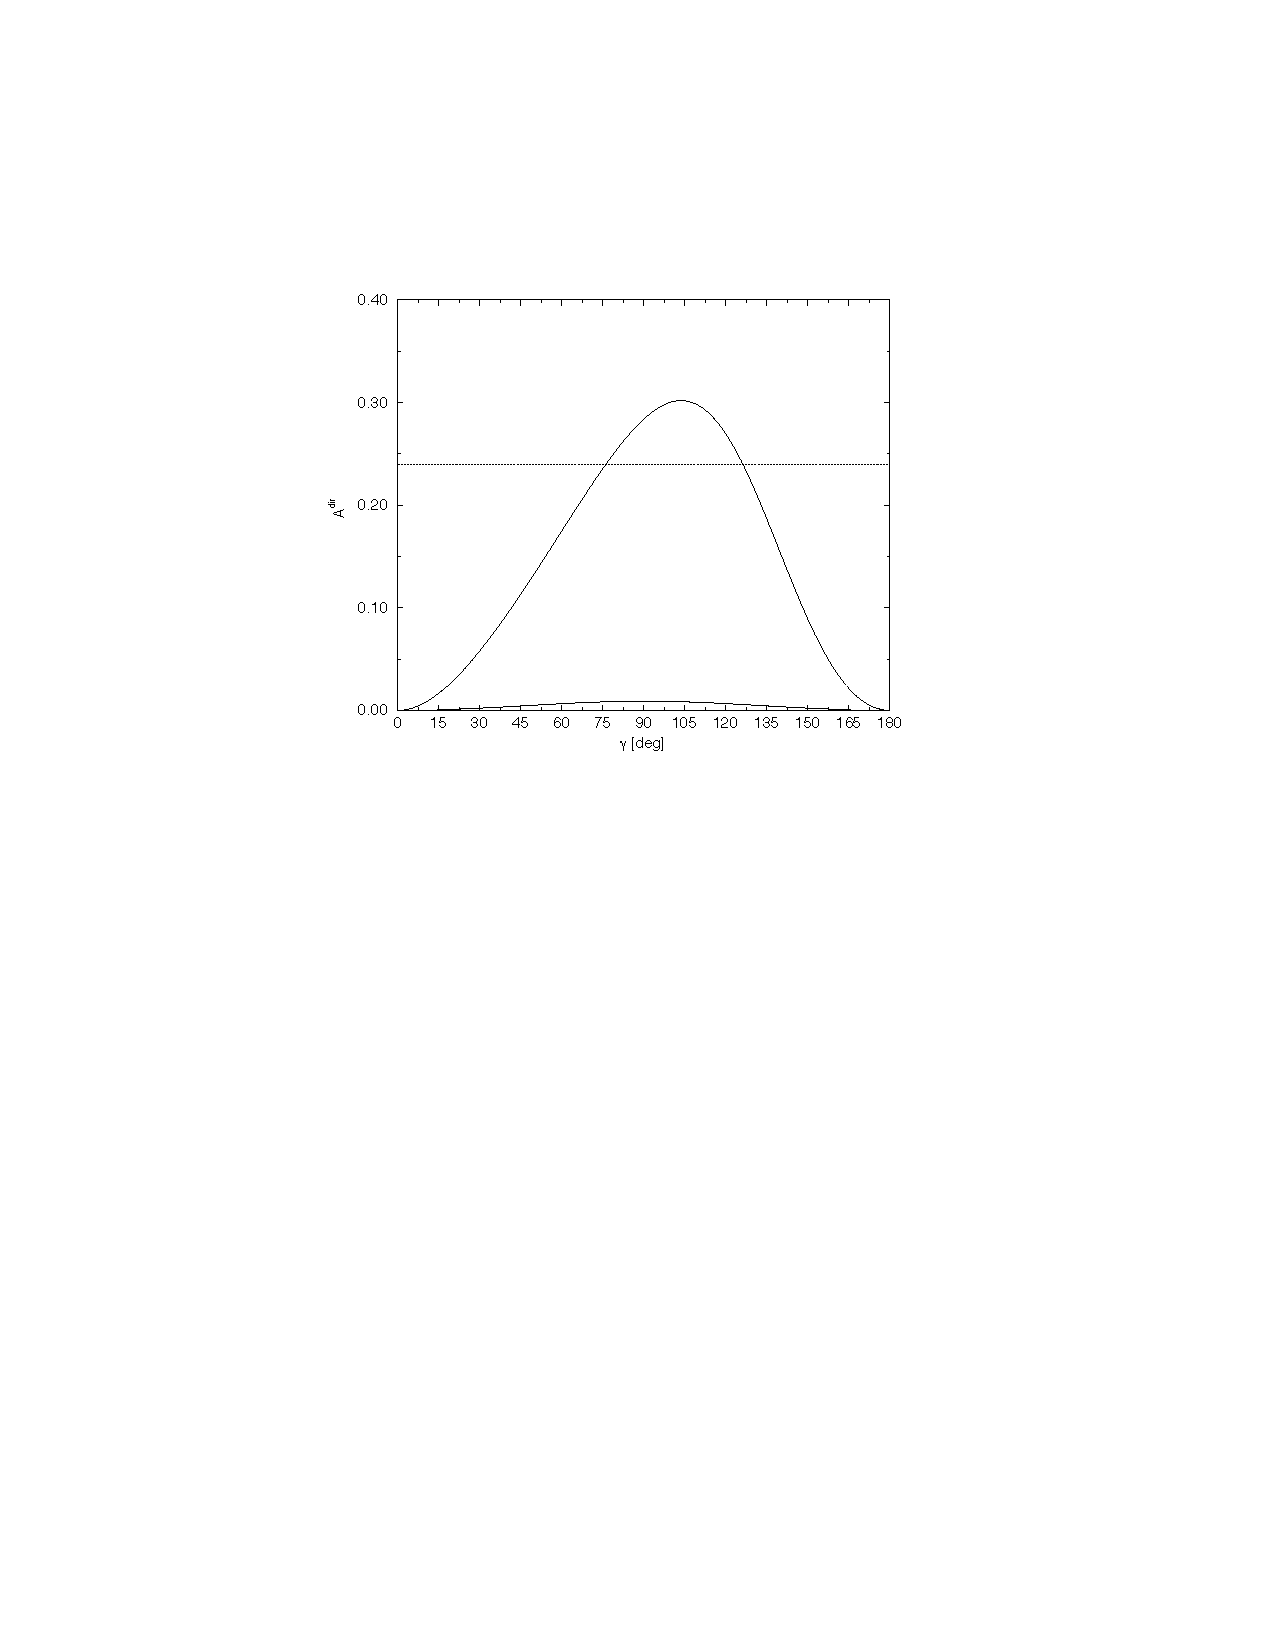
\includegraphics[width=0.4\textwidth]{04gamma/figs/GammaVsCf.pdf}
	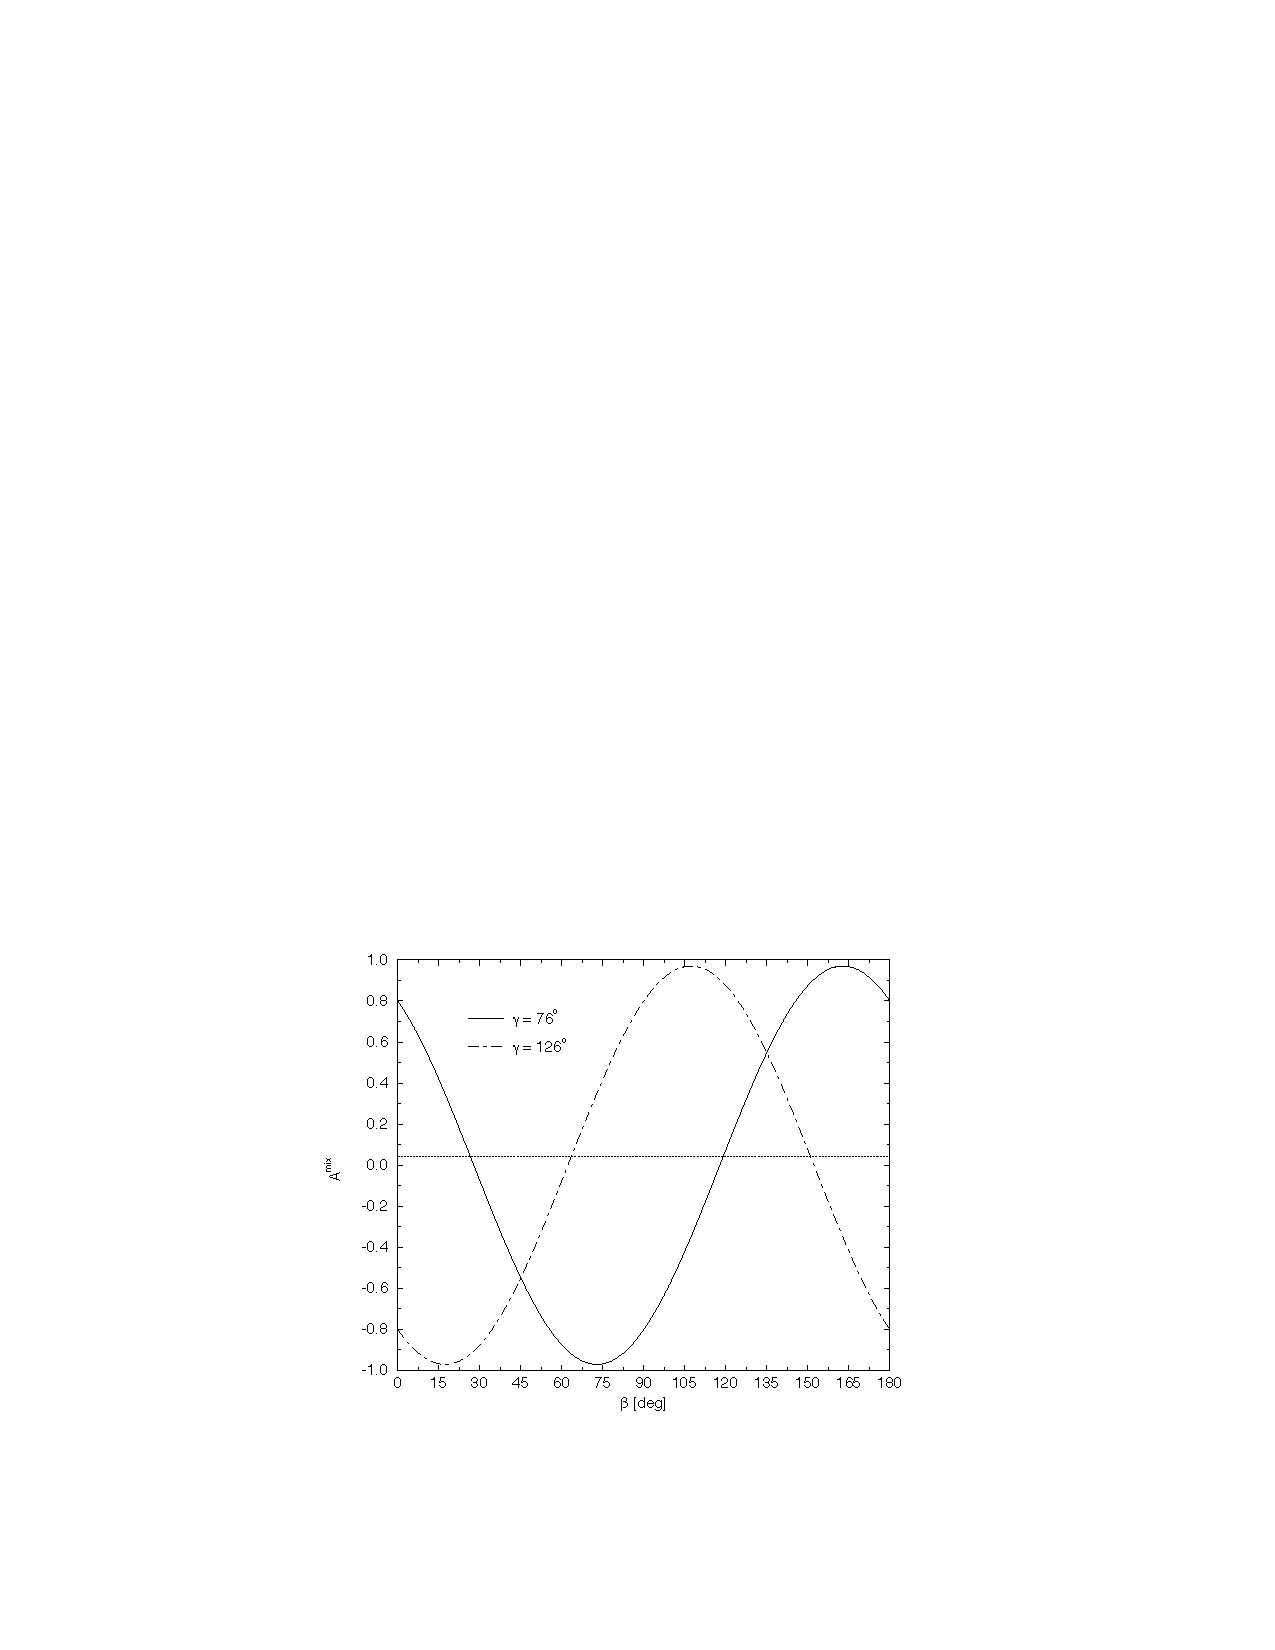
\includegraphics[width=0.4\textwidth]{04gamma/figs/BetaVsSf.pdf}
	\caption{Dependence of $C_{f}^{\Bd\!\to\pip\pim}$ ($A^{\text{dir}}$) on $\gamma$ (left) and $S_{f}^{\Bd\!\to\pip\pim}$ ($A^{\text{mix}}$) on $\beta$ for a specific example as given in \cite{GammaInLoops_Fleischer}.}
	\label{fig:gamma_beta_fleischer}
\end{figure}
Using these two solutions for $\gamma$ and inserting them together with the obtained expressions for $d$ and $\theta$ into $S_{f}^{\Bd\!\to\pip\pim}$ gives additionally a fourfold ambiguity for $\beta$ (see \cref{fig:gamma_beta_fleischer}).
Hereby for both ambiguities the assumption is made, that $\gamma\in[0, 180]\si{\degree}$ and $\beta\in[0, 180]\si{\degree}$.
If additionally the phase $\beta$ is used this ambiguities can be resolved by expressing $d$ and $\theta$ as functions of $\gamma$, $C_{f}^{\Bd\!\to\pip\pim}$ and $S_{f}^{\Bd\!\to\pip\pim}$ and consequently fixing the contours in the $\gamma-d$ plane.
However assuming a \SI{15}{\percent} and \SI{20}{\percent} U-spin-breaking effect on the parameters $d$ and $\theta$, respectively, an additional uncertainty on the extracted value of $\gamma$ of roughly \SI{20}{\percent} could arise \cite{GammaInLoops_Fleischer2}.
Adding also the modes $\Bd\!\to\piz\piz$ and $\Bu\!\to\piz\pip$ allows additionally to either constrain \ac{NP} effects in the $\bquark\!\to\squark$ penguin contributions or in mixing \cite{GammaInLoops_Ciuchini}.

\subsection[head={Comparison of tree-level and loop determinations of $\gamma$},tocentry={Comparison of tree-level and loop determinations of $\gamma$}]{Comparison of tree-level and loop determinations of $\symbfsf{\gamma}$}

Both strategies described in the previous two section have been used to determine the angle $\gamma$.
The potential of determination via tree-level processes was studied in many different final states and is combined on a regular basis into one single determination from \lhcb. The most recent combination was presented in \cite{GammCombo} yielding a result of
\begin{equation}
\gamma=\left(74.0^{+5.0}_{-5.8}\right)\si{\degree}.
\end{equation}

\section[head={Measuring $\gamma$ in $\Bz\to\Dm\pip$},tocentry={Measuring $\gamma$ in $\Bz\to\Dm\pip$}]{Measuring $\symbfsf{\gamma}$ in $\symbfsf{\Bz\to\Dm\pip}$}
\label{sec:GammaInBd2Dpi}
